\chapter{Test e raccolta dati}

I test implementati simulano tre possibili scenari di attacco da parte di uno o più attori malevoli presenti all'interno della rete.\newline
Nel dettaglio si è deciso di analizzare un \textit{DoS} di \textit{filtering}, l'attacco al $51\%$ ed un comportamento di \textit{selfish mining}.\newline
I dati dei vari test sono stati raccolti eseguendo diverse run per ciascun test utilizzando parametri ad-hoc per i singoli scenari. Con l'ausilio di diversi script in Bash e Python3 è stato possibile aggregare i dati e semplificarli al fine di creare alcuni grafici. I log di ogni singola run sono stati categorizzati in base ai parametri per la successiva fase di aggregazione automatica. Tutti i valori relativi al tempo riportati durante la raccolta dati fanno riferimento al tempo simulato, sono, ovvero, il numero di step eseguiti dal simulatore.
Tutti i test sono stati esegui su sistema operativo GNU/Linux ed i grafici sono stati creati utilizzando la libreria Python \href{https://matplotlib.org/}{\texttt{matplotlib}}.
\begin{figure}[H]
    \centering
    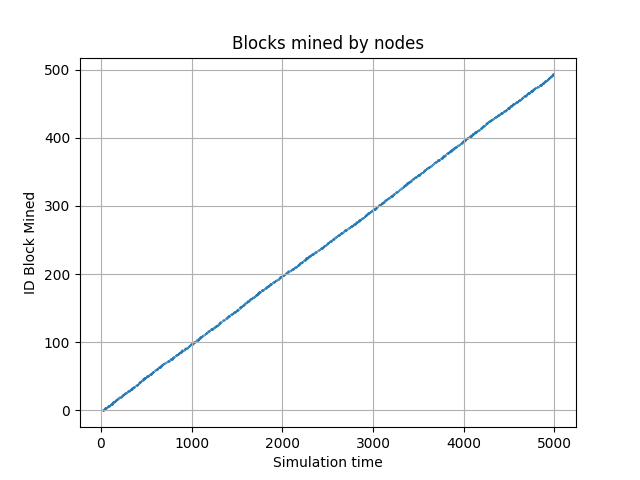
\includegraphics[width=0.65\textwidth]{./images/all-test-51-1.png}
    \caption{Grafico dei blocchi calcolati e diffusi in una rete priva di attaccanti (numero di nodi: $10000$).}
\end{figure}
Una esecuzione di $5000$ step priva di parametri per la simulazione di scenari di attacco con $10000$ nodi impiega circa $60$s per completare.\newline
I parametri utilizzati dalla rete e dal protocollo sono raccolti in Tabella~\ref{tab:parameters}.
\begin{table}[H]
    \resizebox{\textwidth}{!}{\begin{tabular}{|l|l|l|}
        \hline
        \begin{tabular}[c]{@{}c@{}}Nome\end{tabular} &
        \begin{tabular}[c]{@{}c@{}}Valore\end{tabular} &
        \begin{tabular}[c]{@{}c@{}}Descrizione\end{tabular} &
        \hline
        \texttt{TTL}                   & 16                   & \textit{Time-To-Live} utilizzato per ridurre l'overhead \\
        \texttt{DISSEMINATION}         & 7                    & Protocollo di disseminazione dipendente dal grafo \\
        \texttt{PROBABILITY\_FUNCTION} & 2                    & Funzione dipendente dal grafo con scala logaritmica\\
        \texttt{FUNC\_COEFF\_HIGHER}   & 4                    & Parametro più significativo per la funzione\\
                                       &                      & di propagazione dipendente dal grado\\
        \texttt{FUNC\_COEFF\_LOWER}    & 74                   & Parametro meno significativo per la funzione\\
                                       &                      & di propagazione dipendente dal grado\\
        \texttt{END\_CLOCK}            & 5000                 & Numero di step da eseguire \\
        \texttt{MINERS\_COUNT}         & 70                   & Percentuale dei \textit{miner} rispetto al totale dei nodi\\
        \texttt{DIFFICULTY}            & 6489747252517        & Valore della difficoltà della rete \\
        \texttt{HASHRATE}              & 43983561622000000000 & Totale hashrate della rete espresso in \textit{H/s}\\
        \hline
    \end{tabular}}
    \caption{Tabella parametri utilizzati durante le simulazioni.}
    \label{tab:parameters}
\end{table}

\section{DoS}
Il test realizzato va ad analizzare uno scenario un cui uno o più nodi della rete agiscono come dei ``filtri''; una volta individuata una vittima i messaggi da essa generati non vengono inoltrati nella rete se ricevuti da un nodo attaccante.\newline
Questa tipologia di attacco si evolve in un \textit{Sybil Attack} una volta che tutti i nodi malevoli formano un intorno del nodo vittima.\newline
Il test è stato progettato in modo tale che i nodi attaccanti blocchino ogni tipologia di messaggio creata dal nodo vittima. Questo comporta una possibile mancanza di riconoscimento del lavoro di mining e di validazione o pubblicazione delle transazioni.\newline
L'esecuzione del test è stata impostata in modo tale che il numero dei nodi attaccanti aumentasse ad ogni run. Partendo da una rete in cui ci è presente un solo nodo per il \textit{filtering} fino al massimo di $9999$. Il test colleziona i dati riguardanti sia i blocchi generati e propagati sia le transazioni create e diffuse in rete.\newline
La raccolta dei dati prevede, per ogni messaggio generato dal nodo vittima, il conteggio dei nodi, in media, che hanno ricevuto il messaggio. Per ciascuna esecuzione è anche possibile utilizzare i log di output per calcolare e visualizzare il numero di nodi raggiunti da ciascun messaggio, distinto per \texttt{BlockMsg}, \texttt{TransMsg} o \texttt{AskMsg}.
I risultati ottenuti (Figura:~\ref{fig:dos} e Figura:~\ref{fig:dosmix}) sono compatibili con quelli teoricamente aspettati. Il numero di nodi raggiunti in media dai messaggi del nodo vittima decresce proporzionalmente al numero di attaccanti presenti.\newline
Il numero dei nodi raggiunti si azzera e l'attacco ha completamente successo quando il numero degli attaccanti è tale di escludere il nodo vittima dal resto della rete.\newline
È significativo notare, quindi, che la posizione di un nodo e il numero dei peer vicini (\textit{grado}) incide un ruolo fondamentale sulla riuscita o il fallimento dell'attacco. Anche nel caso in cui un solo nodo, non controllato dall'attaccante, propagasse il traffico in uscita dal nodo vittima la rete potrebbe essere ugualmente aggiornata.\newline
\begin{figure}[H]
    \centering
    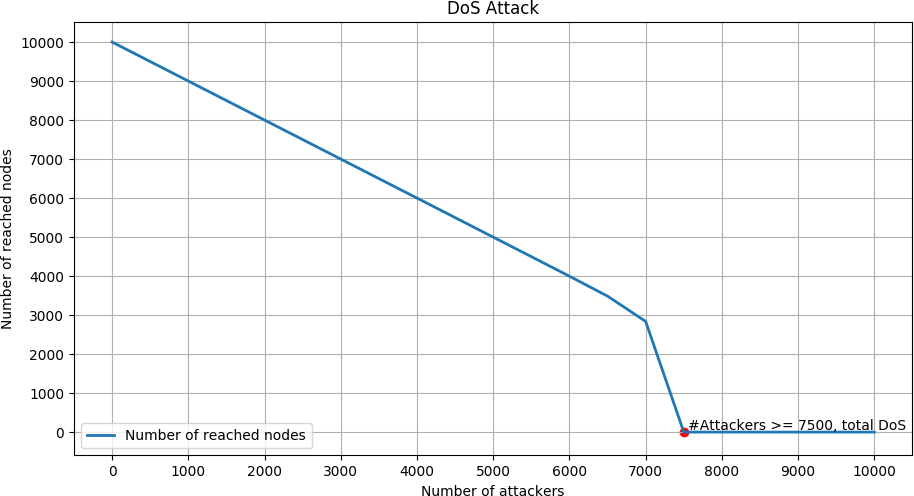
\includegraphics[width=\textwidth]{./images/attackDOS.png}
    \caption{Grafico della media dei nodi raggiunti nelle varie run di test di un attacco \textit{DoS} di tipo \textit{filtering}.}
    \label{fig:dos}
\end{figure}
\begin{figure}[H]
    \centering
    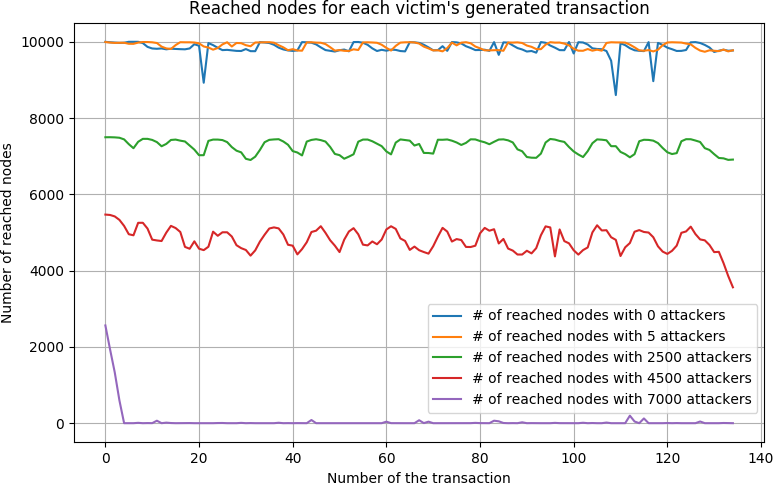
\includegraphics[width=\textwidth]{./images/DOS-mix.png}
    \caption{Confronto del numero di nodi raggiunti per ogni transazione prodotta dal nodo vittima in presenza di diversi numeri di attori malevoli nel caso di \textit{DoS} di tipo \textit{filtering}.}
    \label{fig:dosmix}
\end{figure}
È importante sottolineare che nel protocollo \textit{peer-2-peer} i dati scambiati non sono cifrati ma per un nodo malevolo risulta impossibile cambiare questi dati a proprio vantaggio. Anche intercettando un messaggio, di pubblicazione di un nuovo nodo, la transazione \textit{coinbase} inserita nel blocco risulta essere valida esclusivamente per il reale proprietario della coppia di chiavi utilizzate per generare la signature. Nel caso in cui un nodo malevolo invalidi un blocco od un messaggio sia ha lo stesso risultato del \textit{DoS} di tipo \textit{filtering} appena presentato.\newline
Al fine di testare anche l'utilizzo dei vari algoritmi di propagazione dei messaggi sono state effettuate ulteriori esecuzioni impostando un \texttt{TTL} maggiore ($20$) e l'algoritmo di propagazione \textit{broadcast} (\texttt{DISSEMINATION=0}). Queste configurazioni generano un elevato overhead nella rete ma dovrebbero aiutare il nodo vittima a raggiungere i nodi anche in situazioni critiche.
\begin{figure}[H]
    \centering
    \includegraphics[width=\textwidth]{./images/DOS-mixv2.png}
    \caption{Confronto del numero di nodi raggiunti per ogni transazione prodotta dal nodo vittima in presenza di diversi numeri di attori malevoli nel caso di \textit{DoS} di tipo \textit{filtering} con algoritmo di propagazione a \textit{broadcast}.}
    \label{fig:dosmix}
\end{figure}

\section{51\% Attack}
L'attacco al $51\%$ apre molteplici scenari in cui uno o più \textit{miner}, in possesso della maggior parte dell'hashrate totale, contribuiscono in maniera esclusiva all'aggiunta dei blocchi nella blockchain primaria. Controllando quali blocchi sono aggiunti alla blockchain un attaccante è in grado di bloccare la conferma delle transazioni e quindi di pagamenti tra utenti e poter effettuare un \textit{double spending}.\newline
Con questo test si vuole osservare come con all'aumentare della potenza di \textit{mining} un attaccante possa prendere il sopravvento sull'intera rete.\newline
\begin{figure}[H]
    \centering
    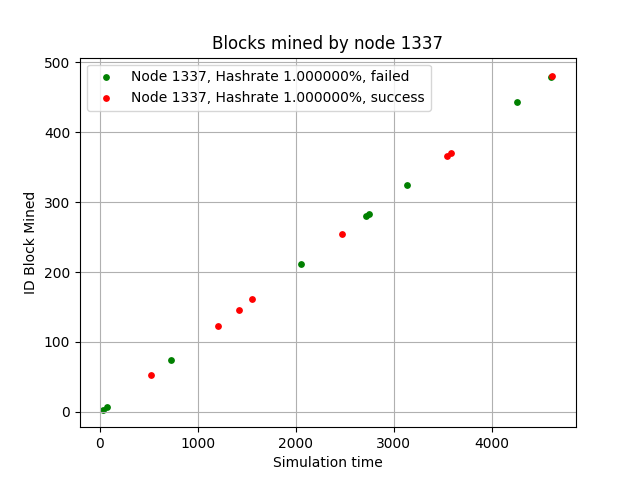
\includegraphics[width=\textwidth]{./images/1337-test-51-1.png}
    \caption{Grafico dei blocchi calcolati e diffusi nella rete dall'attaccante (nodo $1337$) con il $1\%$ dell'hashrate totale.}
    \label{fig:51v1.1}
\end{figure}
I test sono stati strutturanti variando il numero di \textit{miner}, l'hashrate della rete e quello di un nodo attaccante. Prendendo singolarmente il nodo attaccante è possibile osservare l'andamento dei lavoro di \textit{mining}: l'attaccante ha successo quando il blocco da esse pubblicato raggiunge la maggior parte dei nodi. In questo caso non si è interessati al numero di transazioni create, ricevute od inserite nella blockchain ma solo al numero di blocchi trovati; per questo al fine di aumentare le performance e ridurre i tempo di esecuzione sono state disabilitate queste funzionalità.\newline
Una prima versione dell'attacco è stata lanciata configurando la rete con i parametri della Tabella~\ref{tab:parameters} e la potenza di calcolo dell'attaccante crescente dall'$1\%$ al $100\%$.
\begin{figure}[H]
    \centering
    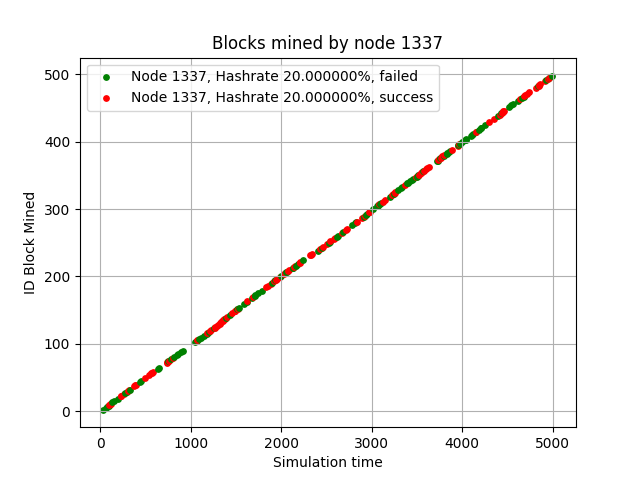
\includegraphics[width=\textwidth]{./images/1337-test-51-20.png}
    \caption{Grafico dei blocchi calcolati e diffusi nella rete dall'attaccante (nodo $1337$) con il $20\%$ dell'hashrate totale.}
    \label{fig:51v1.20}
\end{figure}
Come è possibile vedere dalle due immagini precedenti (Figura~\ref{fig:51v1.1} e Figura~\ref{fig:51v1.20}) all'aumentare dell'hashrate dell'attaccante aumenta anche il numero di nodi prodotti ma ciò non garantisce che i nodi vengano accettati da tutti i nodi in quanto gli altri \textit{miner} potrebbero aver pubblicato il blocco prima o aver raggiunto la maggior parte dei nodi in minor tempo.\newline
Elaborando tutti i dati delle esecuzioni è possibile visualizzare l'andamento tra hashrate e percentuale di successo dell'attaccante (Figura~\ref{fig:51v1}).
\begin{figure}[H]
    \centering
    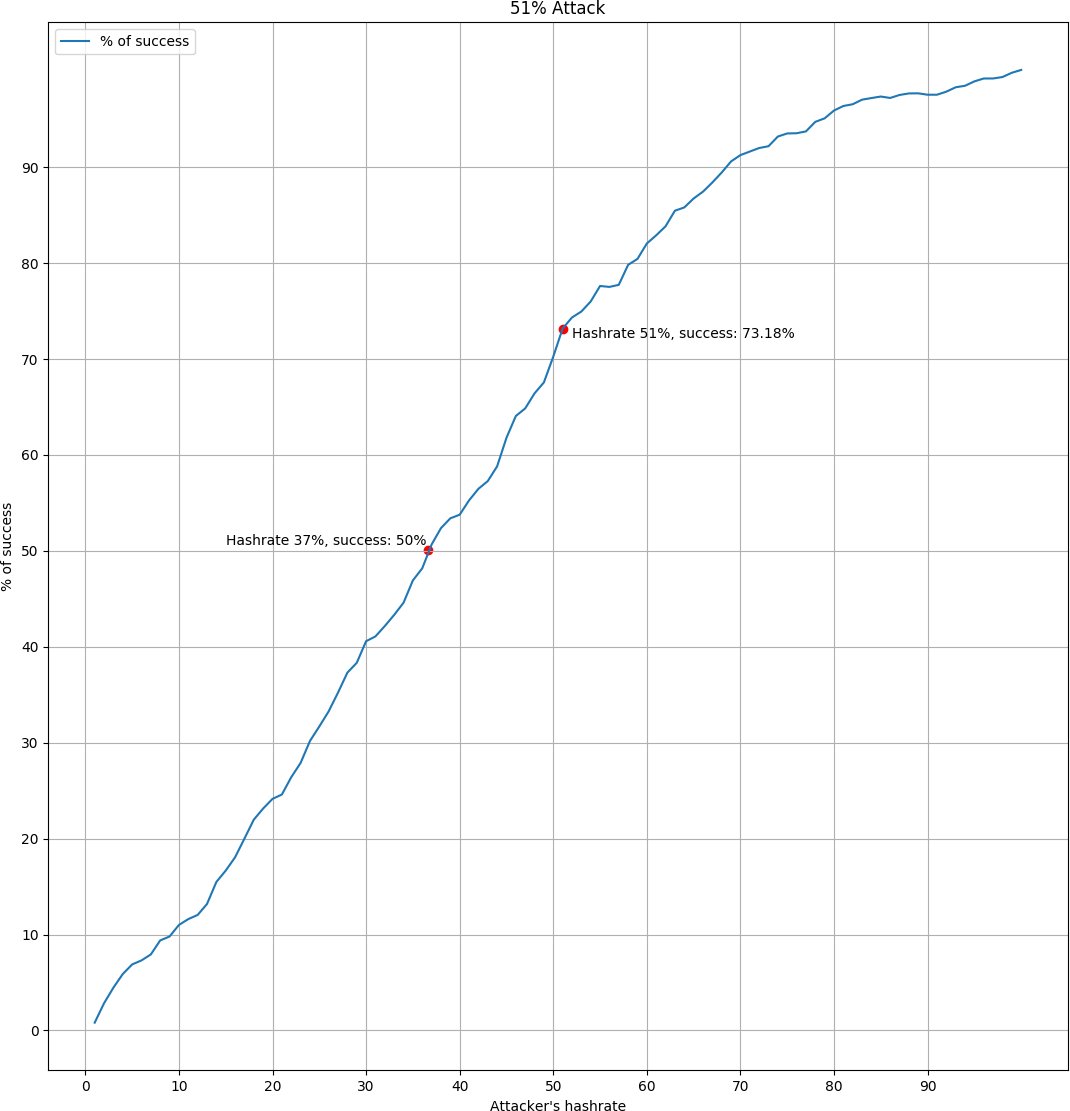
\includegraphics[width=\textwidth]{./images/51-v1.png}
    \caption{Attacco del $51\%$, versione 1.}
    \label{fig:51v1}
\end{figure}
Sorprendentemente le percentuali di successo sono molto elevate anche per hashrate ben la di sotto del $51\%$. Per la soglia del $51\%$ sia che la possibilità di successo è molto alta ($73.18\%$); la facilità dell'attacco questo è dovuto ad una errata modellazione del test: il $70\%$ di \textit{miner} della rete è troppo elevata e questo comporta un hashrate per nodo estremamente basso. La media dell'hashrate per i nodi è dello $0.0142\%$; tale configurazione aumenta notevolmente le possibilità di successo per l'attaccante in quanto non esistono dei \textit{miner} capaci di contrastare una potenza di hashrate molto alta. Anche solo l'$1\%$ risulta essere $70$ volte superiore alla media.\newline
Un secondo tentativo (Figura~\ref{fig:51v2}) è stato effettuato riducendo al $20\%$ il numero di miner.
\begin{figure}[H]
    \centering
    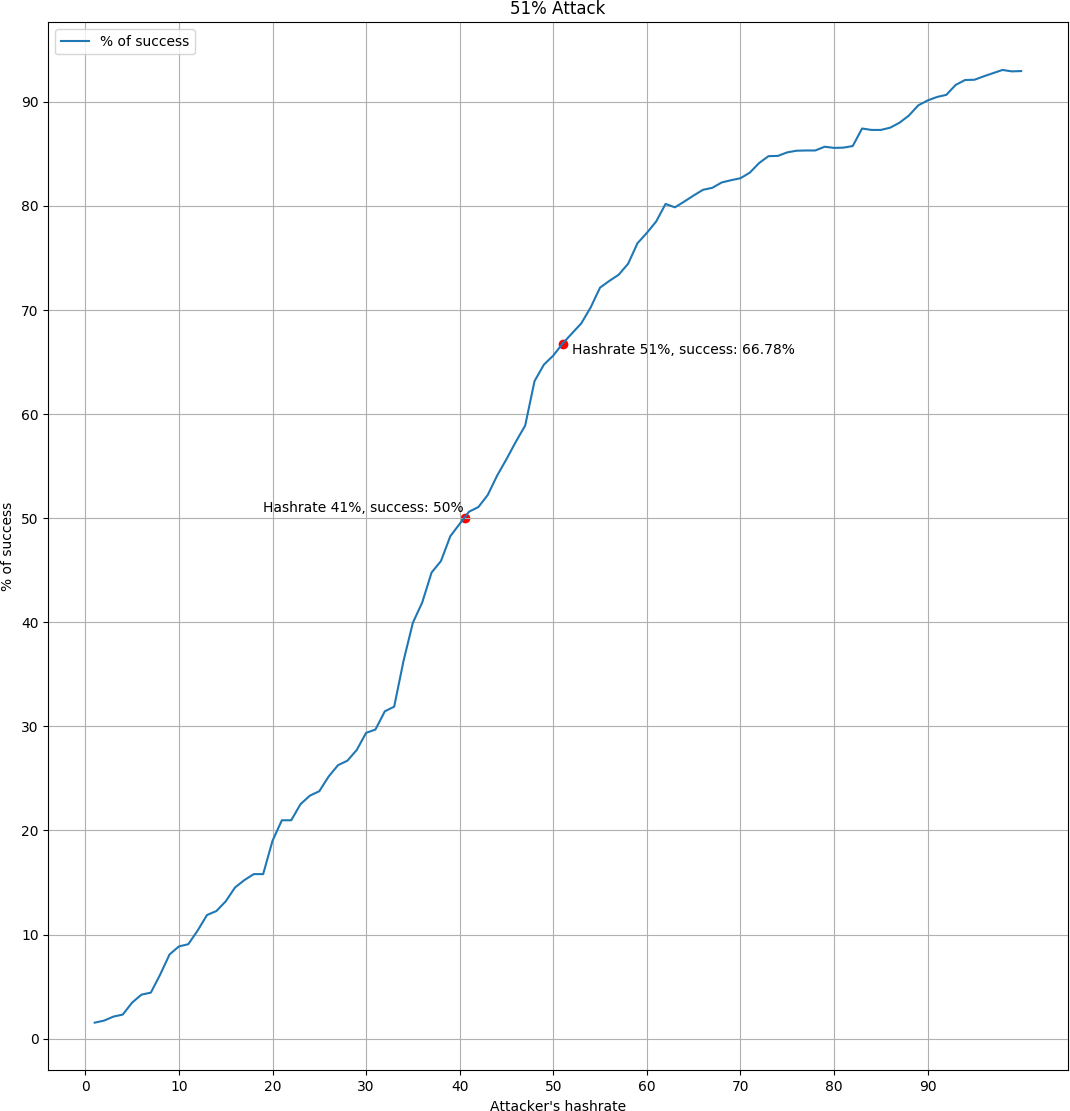
\includegraphics[width=\textwidth]{./images/51-v2.png}
    \caption{Attacco del $51\%$, versione 2.}
    \label{fig:51v2}
\end{figure}
Anche in questo caso i risultati sono sempre molto a favore dell'attaccante ma la riduzione dei \textit{miner} ha incrementato la media dell'hashrate per ogni nodo contrastando l'attaccante.\newline
Infine, è stato eseguito un test con $15$ \textit{miner} ed un ulteriore miglioramento: l'hashrate dell'attaccante non è calcolato in percentuale all'intera rete ma viene sommato al totale. L'hashrate totale della rete con un attaccante con una potenza di calcolo del $20\%$ è del $120\%$. In un caso reale l'attaccante deve inserirsi nella rete con il massimo della potenza che dispone al fine di evitare sia una riorganizzazione della rete e della community sia un aumento della difficoltà dovuta all'aumento totale dell'hashrate.
\begin{figure}[H]
    \centering
    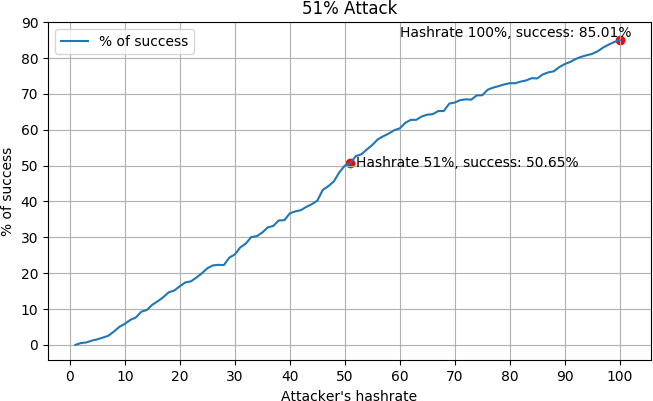
\includegraphics[width=\textwidth]{./images/51-v3.png}
    \caption{Attacco del $51\%$, versione 3.}
    \label{fig:51v3}
\end{figure}
Riducendo quindi sia numero di \textit{miner} totali e strategia dell'attaccante è possibile vedere (Figure~\ref{fig:51v3}) come effettivamente la soglia del $51\%$ garantisca all'attaccante un successo di poco superiore al $50\%$. Un altra osservazione va fatta in quanto anche al $100\%$ della potenza di calcolo (ovvero il $200\%$ della totale) l'attaccante non abbia mai il massimo delle possibilità di successo.\newline
Questo attacco deve essere visto come un gradiente e non come una soglia in quanto anche con soglie di hashrate minori del $51\%$ le probabilità di successo non sono trascurabili. Con gli attuali valori di hashrate (Novembre 2018) il costo per ottenere il $51\%$ di potenza per un'ora tramite cloud computing è di $14~682~645$\$\footnote{\href{https://www.crypto51.app/}{crypto51.app}}. In un'ora vengono pubblicati circa $10$ blocchi per un possibile \textit{reward} totale di $125$ BTC, ovvero $793~625$\$, che potrebbe essere utilizzato per ammortizzare il costo iniziale. Nonostante la possibilità di guadagno ottenuti dai \textit{reward} e da eventuali \textit{double spending} effettuati in un'ora di tempo, è altamente improbabile che qualcuno investa la cifra di $13~889~020$\$ per ottenere poco più del $50\%$ di possibilità di successo.


% NeoTex: mainfile=main.tex:
